\documentclass{standalone}
\usepackage[utf8]{inputenc}
\usepackage[dutch]{babel}
\usepackage[T1]{fontenc}
\usepackage{lmodern}
\usepackage{tikz}
\usetikzlibrary{positioning,mindmap,trees,backgrounds}
\usepackage{hyperref}
\usepackage{microtype}
\definecolor{darkblue}{RGB}{33,26,82}
\definecolor{lightblue}{RGB}{194,193,204}
\begin{document}
\sffamily
	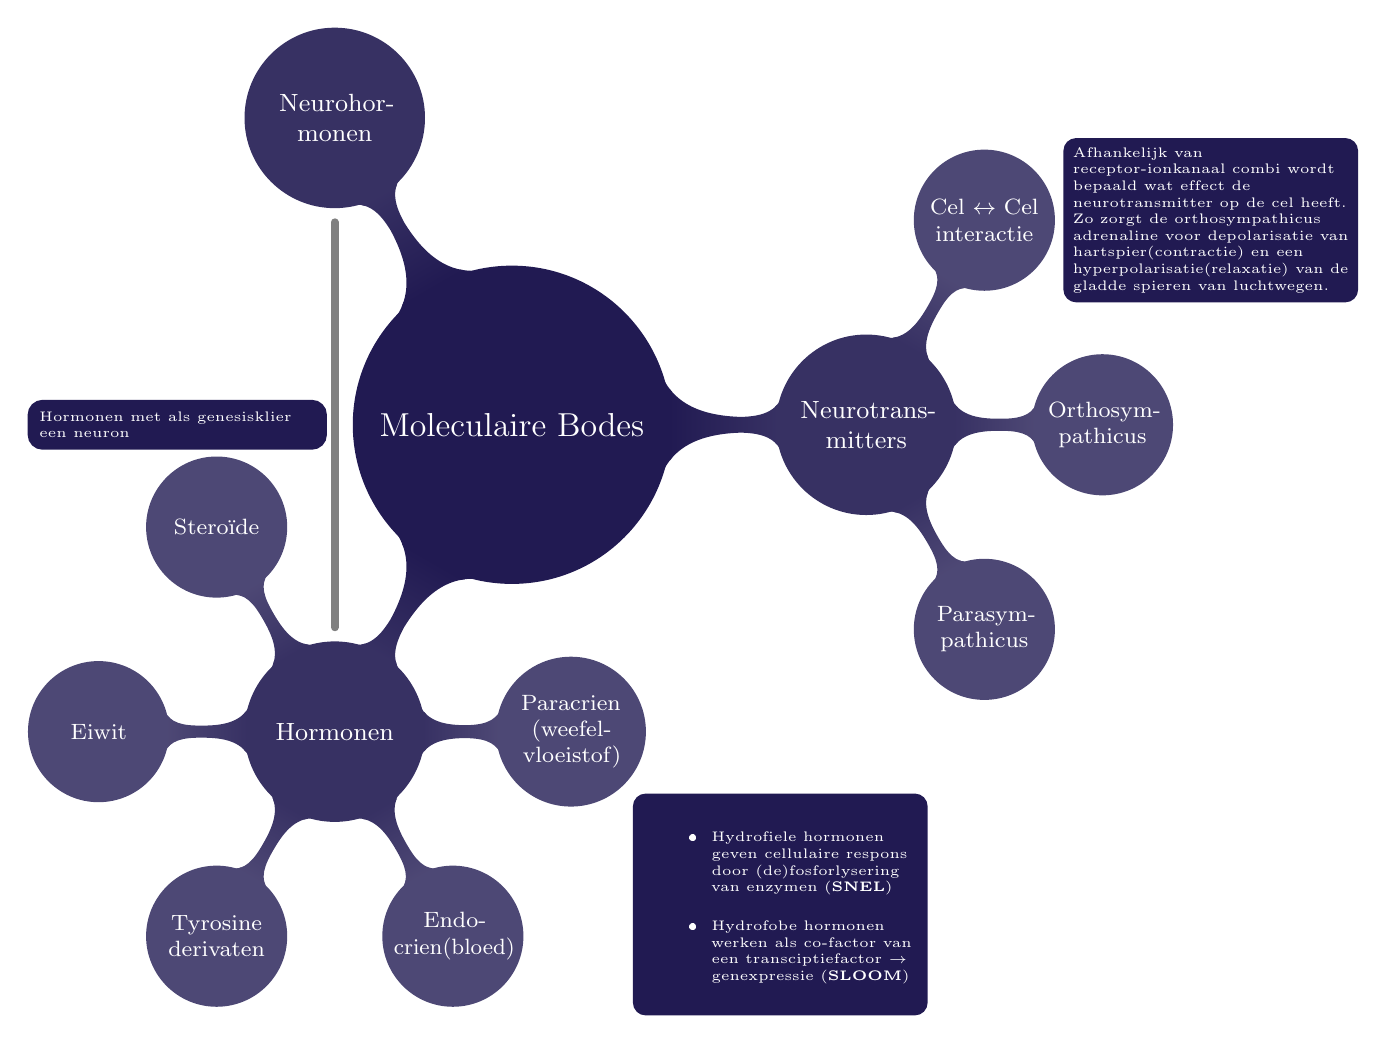
\begin{tikzpicture}[mindmap, 
			every node/.style={concept,execute at begin node=\hskip0pt, 
			text=white},
			grow cyclic,
			level 1/.append style={level distance=4.5cm,sibling angle=120},
			level 2/.append style={level distance=3cm,sibling angle=60},
			concept color=darkblue
			]
		\node(hoofd) {Moleculaire Bodes}
			child[concept color=darkblue!90] {node (a1) {Hormonen}
				child[concept color=darkblue!80] {node (b1) {Stero\"ide}}
				child[concept color=darkblue!80] {node (b2) {Eiwit}}
				child[concept color=darkblue!80] {node (b3) {Tyrosine derivaten}}
				child[concept color=darkblue!80] {node (b4) {Endocrien(bloed)}}
				child[concept color=darkblue!80] {node (b5) {Paracrien \\(weefel-\\vloeistof)}}
		}
			child[concept color=darkblue!90] {node (a2) {Neurotransmitters}
				child[concept color=darkblue!80] {node (b6) {Parasympathicus}}
				child[concept color=darkblue!80] {node (b7) {Orthosympathicus}}
				child[concept color=darkblue!80] {node (b8) {Cel $\leftrightarrow$ Cel interactie}}
			}
				child[concept color=darkblue!90] {node (a3) {Neurohormonen}
			};
		\node[annotation,anchor=north west] at (b5.south east) {\begin{itemize}
					\color{white}
					\item Hydrofiele hormonen geven cellulaire respons door (de)fosforlysering van enzymen (\textbf{SNEL})
					\item Hydrofobe hormonen werken als co-factor van een transciptiefactor $\rightarrow$ genexpressie (\textbf{SLOOM})
				\end{itemize}
				};
			\node[annotation,anchor=west] at (b8.east) {Afhankelijk van receptor-ionkanaal combi wordt bepaald wat effect de neurotransmitter op de cel heeft. Zo zorgt de orthosympathicus adrenaline voor depolarisatie van hartspier(contractie) en een hyperpolarisatie(relaxatie) van de gladde spieren van luchtwegen.};
		\begin{pgfonlayer}{background}
			\draw[concept connection] (a3) -- (a1) node[midway,annotation,anchor=east] {Hormonen met als genesisklier een neuron};
		\end{pgfonlayer}
	\end{tikzpicture}
\end{document}
